\documentclass[a4paper,11pt]{article}
\usepackage{fancyhdr}
\usepackage[utf8]{inputenc}
\usepackage{graphicx}
%\setlength{\headheight}{11pt}

\lhead
\rhead
%\parskip 1em
%\parindent 0em

\begin{document}
\pagestyle{empty}
%-----------------------------------------------------------
\begin{titlepage}

\title{\Huge{Lab report} \\[0.1cm] \Large{Digital Design (EDA322)} \\ [0.4cm] \Large{ \emph{Writing Guidelines}} \\[0.4cm]}
\author{\large{\emph{Group TUE\_PM\_8}} \\[0.2cm] Niklas Gustafsson \\[0.05cm] Oskar Lundström \\[0.1cm]}
\maketitle
\thispagestyle{empty}
\end{titlepage}
\clearpage
%-----------------------------------------------------------
\pagestyle{fancyplain}
\pagenumbering{roman}
\tableofcontents
\clearpage
%%%%%%%%%%%%%%%%
% Introduction
\pagenumbering{arabic}
\setcounter{page}{1}
\section{Introduction}
(max: 1 page)
\\\\
This part will introduce the reader to the report. 

At the beginning, describe what the purpose of this lab report is. Then describe briefly what each section discusses and finally summarize the most important conclusions. 

\section{Method}
\subsection{Arithmetic and Logic Unit (ALU)}
(max: 2 pages)
\\\\
When we built our ALU we began by constructing the most basic component, the full-adder. We started with deriving the boolean expressions for the full-adder. We did this by minimizing the boolean expression for the sum and the carry out signals using a Karnaugh diagram. We came to the conclusion that a full-adder should be built like described in the picture below.
\\
\begin{figure}[h!]
  
\includegraphics[width=\linewidth]{fulladder.png}
  \caption{A full-adder.}
  \label{fig:etikett}
\end{figure}
\\
You can also build a full-adder using two half-adders and some extra logic. This can be done by constructing the circuit below. We came to this conclusion by connecting the resulting signal of the first half-adder to the second one along with the carry in signal. After this we just added the extra logic that was needed, which was an OR gate.
\\
\begin{figure}[h!]
  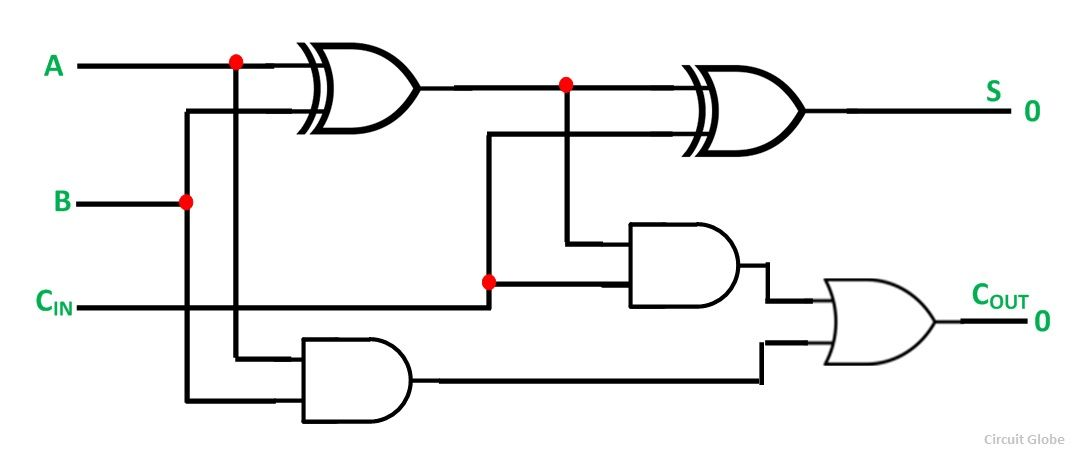
\includegraphics[width=\linewidth]{fulladderfromhalfadder.jpg}
  \caption{A full-adder made from two half-adders.}
  \label{fig:etikett}
\end{figure}
\\\
We created an eight bit ripple carry adder (RCA) by connecting eight full-adders together according to the diagram below. The idea is to simply connect the carry out signal of the first full-adder to the carry in signal of the second one, and so on. The RCA was used in our original design of the ALU but later we replaced it with a carry lookahead adder (CLA) which we constructed according to the instructions in the optional task of lab 2. 
\\
\begin{figure}[h!]
  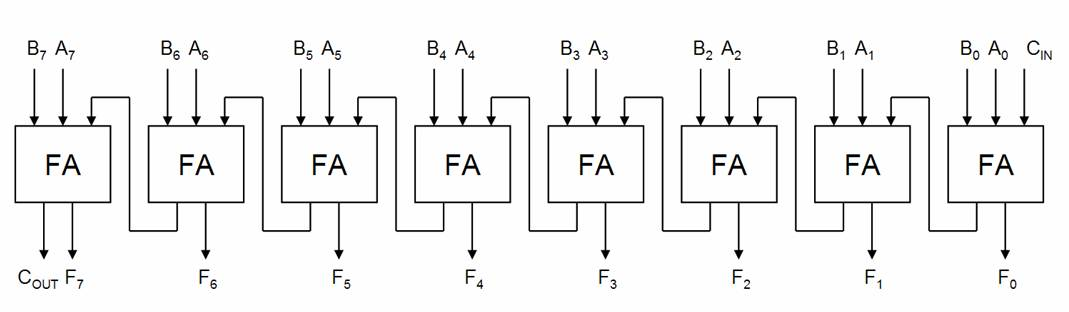
\includegraphics[width=\linewidth]{rca.jpg}
  \caption{A ripple carry adder.}
  \label{fig:etikett}
\end{figure}
\\
The ALU includes a comparator unit which is used to check whether the operands are equal or not. There are two ways to implement this comparator, by using the structural or dataflow style of VHDL. We decided to do the dataflow implementation because we thought it would be easier and that it would result in a more clean code. In order to check whether the operands are not equal we performed a bitwise XOR on the operands and checked if the resulting bitstream was zero. This was used as the resulting NEQ signal. The EQ signal was simply an inversion of the NEQ signal. 
\\\\
If we were to do this in structural VHDL we would have to create a component which cheked if two certain bits were not equal. We would then have to create eight such components and perform an OR operation on the results. If that result would be zero they would not be equal. This result would've been used as the NEQ signal and an inversion of it would be used as the the EQ signal. 
\\\\
Our ALU supports subtraction between the operands. The operation A minus B is performed by converting B to its 2-compliment and then adding it with A. In order to get the 2-compliment representation for B we invert all the bits of B and set the carry in signal to one. In order for this to be possible we need to add eight XOR gates (one for each bit in B). The input to these XOR gates are the respective bits of B and the SUB signal. The SUB signal is one when the operation signal is set to subtraction. The SUB signal is also connected to the carry in signal, I.E the carry in is set to one whenever we subtract according to above. In this way we can easily perform the operation A - B by setting the operation signal to subtraction and enter A and B as usual.
\\\\
* PICTURE OF LOGIC *

\noindent
\textbf{Findings and observations}

One thing that we learned was that in VHDL the entity names in a project have to be unique for all references to work properly. 

We also learnt why the critical path for an n-bit RCA is $2n+1$ gates. For every full adder the carry-out depth depends on the inputs ($3$ gates deep) and the carry-in ($2 + $previous depth). The depth is the maximum of these. For the first the depth becomes $3$, for the second $5$ and so on. In other words, for the first adder the inputs are the fartherest away, but for the following it is the carry-in instead. \\


\\
One thing that we learned was that in VHDL the entity names in a project have to be unique for all references to work properly. 

Another thing we learnt was that the critical path for an n-bit RCA is $2n+1$ gates. The last carry-out is the longest. For every full-adder the carry out needs the carry-in (passes 2 gates) and the inputs (passes 3 gates). The first adder can pass on its carry-out after 3 gates. But the second adder can pass on its carry-out after just 2 more steps since the result from the inputs have already arrived to the last AND gate.
\\
\\
TO BE REMOVED
Describe what you did in lab 2 and what you have learnt. In addition, discuss your findings and observations during this lab. Summarize your answers to the questions in the lab PM and present the block diagrams that you have drawn. Furthermore, describe how your ALU performs subtraction using an adder. Remember to always explain your design choices and mention any assumptions. Finally, make use of figures and tables. 

\subsection{Top-level Design}
(max: 2 pages)
\\\\
Describe what you did in lab 3. In addition, describe how you implemented the bus using the mux and any extra logic or the tri-state buffers. Describe briefly how you implemented the storage elements that are used by the ChAcc processor. Show one snapshot of the simulation waveform where you write something to a memory location and then read from it. Remember to always explain your design choices and mention any assumptions. Finally, make use of figures and tables. 

\subsection{Controller}
(max: 2 pages)
\\\\
Describe what you did in lab4. More specifically, show the \emph{Finite-state machine} (FSM) of the controller by presenting the diagram you drew. Which design decisions did you make and why? Also include few waveforms, where you show that the controller runs correctly for some particular instructions using the provided testbench. Remember to always explain your design choices and mention any assumptions. Finally, make use of figures and tables. 

\subsection{Processor's Testbench}
(max: 2 pages)
\\\\
Describe what you did in lab5. More specifically, describe how you made the testbench to verify that your processor design was functionally correct. For example, you can specify how you generated inputs to the processor during the testing, how you were reading the expected outputs and how you compare the expected outputs with the actual outputs. Also mention if your processor design was working correctly from the beginning and if not describe how you backtrack the bugs. Remember to always explain your design choices and mention any assumptions. Finally, make use of figures and tables. 

\subsection{ChAcc on Nexys 3 board \emph{(Optional)}}
(max: 2 pages)
\\\\
Describe how you verified the correctness of your FPGA implementation. Note that the code that is executed on the implementation is the same code used for testing in Lab 5. You should compare sequences of values on various signals observed on the seven-segment displays to values seen in Modelsim simulation of the design. Please include in the report the sequence of program counter (PC) and display register values you observed during a successful execution on the FPGA. 

\subsection{Performance, Area and Power Analysis \emph{(Optional)}}
(max: 2 pages)
\\\\
To be announced in the Lab7PM.

\section{Analysis}
(max: 1 page)
\\\\
Summarize your results after performing all the labs (2, 3, 4 and 5).

Mention and discuss interesting findings and observations, as well as difficulties in completing some of the tasks of the four last labs.

After looking at your results, draw conclusions and describe briefly the learning outcome, that is what have you learnt by performing these labs?  

% Appendix
\newpage
\begin{appendix}

\section{Appendix}
(max: 4 pages)
\\\\
In the appendix, you can include extra figures or tables that don't fit in the main body of the lab report. 

\end{appendix}

\end{document}
